\section{Theory}\label{sec:theory}

In this section, we will discuss the theoretical foundations of message passing neural networks (MPNNs) and ensembles for predicting
the binding energy of molecules in a catalyst process. The section will start with a note on symmetry, specifically detailing the
usage of invariant and equivariant representations in the model. Moving on to a detailing of the modelling architecture, ending in a
presentation of the ensemble structure and metrics used in the experiment.

\subsection{Symmetry}\label{sec:symmetry}
A large part of the contribution from the PAINN paper\cite{PAINN}. is the emphasis on building and modelling equivariant features.
The interest in equivariance, comes from the ability to express more information about a graph structure, at a lower level of
computational cost. This ties in with the search for modelling approaches that descrease lead-time on predictions, while maintaining an
acceptable error-rate.
let $\vec{\mathbf{x}}$ be a feature, and $o$ denote an operation.
$\vec{\mathbf{x}}$ is a rotational equivariant feature, under the operation $o$,
if the below equation is satisfied for any rotation matrix $R \in \mathbb{R}^{3 \times 3}$\ref{eq:equivariant}:

\begin{equation}\label{eq:equivariant}
    R \vec{\mathbf{o}}(\vec{\mathbf{x}}) = \vec{\mathbf{o}}(R \vec{\mathbf{x}})
\end{equation}

And $\vec{\mathbf{x}}$ is a rotational invariant feature, under the operation $o$,
if the below equation is satisfied for any rotation matrix $R \in \mathbb{R}^{3 \times 3}$\ref{eq:invariant}:

\begin{equation}\label{eq:invariant}
    \mathbf{o}(\vec{\mathbf{x}}) = \mathbf{o}(R \vec{\mathbf{x}})
\end{equation}

In order to detail whether any of these equations hold, one needs to consider which operations, make this the statements true for
directional information. The paper of inspiration \cite{PAINN} highlights a list of operations,
that equivariant MPNN's in particular can use in order to preserve equivariant information properties on their features:

\begin{itemize}
    \item Any (nonlinear) function of scalars: $\mathbf{f}(\mathbf{s})$
    \item Scaling of vectors $ \mathbf{s} \circ \vec{\mathbf{v}}$
    \item Linear combinations of equivariant vectors: $\mathbf{W} \vec{\mathbf{v}}$
    \item Scalar products: $\mathbf{s} = \left \| \vec{\mathbf{v}} \right \|^{2}, s = \left \langle \vec{\mathbf{v}}_{1}, \vec{\mathbf{v}}_{2} \right \rangle$
    \item Vector products: $\vec{\mathbf{v}}_{1} \times \vec{\mathbf{v}}_{2}$
\end{itemize}

This list entails a linearity constraint on the operations on equivariant features\cite{PAINN}. If the linearity constraint is
not satisfied, then the feature will not be equivariant, and directional information will not be preserved.

The subsequent section presents
a number of features (presented also as representations below) and operations relevant to the MPNN.
These need not all be equivariant, invariant, linear or non-linear. What constitutes an equivariant MPNN in the eyes of
Schütt et. al.\ref{PAINN}, is not that all operations on directional information are linear, and equivariance is preserved globally.
As long as an equivariant representation containing directional information, is obeying  the constraints of the list above and thereby
equation\ref{eq:equivariant}, directional information is preserved, and can be allowed to diffuse through the model representations.

\subsection{Message Passing Neural Networks}\label{subsec:modelling_task}

The key idea behind MPNNs is the concept of
message passing, where each node in the graph exchanges information with its neighbors in an iterative manner.

Let $G = (N, E)$ be a graph, where $N$ is the set of nodes and $E$ is the set of edges.
Each node $n \in N$ is associated with an invariant representation vector $\mathbf{S}_{n} \in \mathbb{R}^{Fx1}$,
an equivariant representation
vector $\vec{\mathbf{v}}_{n} \in \mathbb{R}^{Fx3}$ and a position in 3D space $\vec{r}_{i} \in \mathbb{R}^3$.
$F$ denotes the number of features in the state representation (in our case, $F = 64$ and $F = 128$).
Each edge $(i, j) \in E$ is associated with vector difference $\vec{r}_{ij} = \vec{r}_{i} - \vec{r}_{j}$.
A node $n_{j} \in N$ is said to be a neighbour of a node $n_{i} \in N \setminus \{n_{j}\} = \mathcal{N}(i) $
if $n_{j}$ is within the cutoff distance of $n_{i}$: $\mathcal{N}(i) = \{j |\lVert \vec{r}_{ij} \rVert \leq r_{cut}  \}$.


The message passing process in an MPNN can be described by the following equations \ref{eq:message_block} and \ref{eq:update_block}
following the notation of \cite{PAINN}.

\begin{equation}\label{eq:message_block}
    \vec{\mathbf{m}}_{i}^{v,t+1} = \sum_{j \in \mathcal{N}(i)} \vec{M_t}(\mathbf{S}_{i}^{t}, \mathbf{S}_{j}^{t}, \vec{\mathbf{v}}_{i}^{t}, \vec{\mathbf{v}}_{j}^{t}, \vec{r}_{ij})
\end{equation}

\begin{equation}\label{eq:update_block}
    \vec{\mathbf{s}}_{i}^{v,t+1} = \vec{U_t}(\mathbf{S}_{i}^{t}, \vec{\mathbf{v}}_{i}^{t}, \vec{\mathbf{m}}_{i}^{v,t+1})
\end{equation}

The $U$ and $M$ functions respectively being the update, and message functions, taking into account scalar, vector and
directional features. These equations utilize both invariant and equivariant representations, letting
representations interact, in accordance with knowledge surrounding the chemical descriptor trying to be predicted. The underlying
operations of the functions $U$ and $M$, have a linearity constraint on equivariant representations of directional information,
in order to maintain
information, throughout the modelling process\cite{Atz2021}. The message and update functions will be designed, such that scalars $\mathbf{s}_{i}$
and vectors $\vec{\mathbf{v}}_{i}^{t}$ are updated in an iterative manner via the output residuals $(\Delta \mathbf{s}_{i}^{t}, \Delta \vec{\mathbf{v}}_{i}^{t})$ produced by the message and update functions.
this entails that for the message block output is:

\begin{equation}\label{eq:residual_message}
    \sum_{j \in \mathcal{N}(i)} \vec{M_t}(\mathbf{S}_{i}^{t}, \mathbf{S}_{j}^{t}, \vec{\mathbf{v}}_{i}^{t}, \vec{\mathbf{v}}_{j}^{t}, \vec{r}_{ij}) = (\Delta \mathbf{s}_{i}^{m}, \Delta \vec{\mathbf{v}}_{i}^{m})
\end{equation}

And for the update block output is:

\begin{equation}\label{eq:residual_update}
    \vec{U_t}(\mathbf{S}_{i}^{t}, \vec{\mathbf{v}}_{i}^{t}, \vec{\mathbf{m}}_{i}^{v,t+1}) = (\Delta \mathbf{s}_{i}^{u}, \Delta \vec{\mathbf{v}}_{i}^{u})
\end{equation}

These residuals will be further developed in the sections coming.


\subsubsection{Message Block}\label{subsubsec:message_block}

Further, we define the residual update of invariant scalar\ref{eq:residual_scalar}-representations in the message block,
based on the expression derived earlier in equation\ref{eq:residual_message}:

\begin{equation}\label{eq:residual_scalar}
    \Delta \mathbf{s}_{i}^{m}= (\phi_{s}(\mathbf{s}) * \mathcal{W}_{s})_{i} = \sum_{j} \phi_{s}(\mathbf{s}) \circ \mathcal{W}_{s} \left ( \left \| r_{ij} \right \| \right )
\end{equation}

Worht mentioning about the above expression, are that the index 's' refers to a certain split of the $\phi \circ W$-product seen
in figure\ref{img:message_block}. All indexes of 's', 'v', or a combination of the two in the below equations,
will be detailing what part of a split it belongs to. This comes down to $\phi$ and $\mathcal{W}$ being shared networks, that are re-used
for multiple parts of the modelling.
Following the above equation\ref{eq:residual_scalar}, two expression are utilized, namely $\phi_{s}$ and $\mathcal{W}_{s}$.
$\phi_{s}$ represents atomwwise layers, which have undergone transformations through two linear layers and a SiLU-function,
introducing some non-linearity potentially for better gradient flow, via the smooth gradient. Conceptually it can be interpreted as an
expansion of the embedded atomwise neighbours of a node.
Let $f(x)$ denote a linear layer:

\begin{equation}\label{eq:linear_layer}
    f(x) = w \cdot x + b
\end{equation}

and $SiLU(x)$ denote the SiLU-function:

\begin{equation}\label{eq:SiLU}
    SiLU(x) = x \cdot \left (  \frac{1}{(1+e^{-x}))}\right )
\end{equation}

Then $\phi$ is defined as:

\begin{equation}\label{eq:phi}
    \phi_{s}(\mathbf{s}) = f_{1}(SiLU(f_{2}(\mathbf{s})))
\end{equation}

Worth noting about the above equation\ref{eq:phi}, are the indexes of the linear layers. These are maintained to emphasize,
the individuality of their parameters throughout the whole modelling process.

The rotationally invariant filters $\mathcal{W}_{s}$ are defined as, are linear combinations of a radial basis function
(RBF)\ref{eq:rbf}\cite{Atz2021}. The radial basis function outputs are chosen such that it is centered around twenty
points, $ C = \{1, 2, 3, \ldots, 20\}$. These twenty points are centers of the filter, and their units are Angstrom.
These centers are chosen, such that they cover all distances in the data set, which is confirmed in a later section\ref{distances}.
The expansions provide a representation of similarity or dissimilarity, between the input relative position $\vec{r}_{ij}$,
and the chosen points $C$ \cite{rbf}.
The function takes directional information $\lVert \vec{r}_{ij} \rVert$ and a cutoff
$r_{cut}$. The rbf acts as filter generating function\cite{Schütt2017},
effectively quantizing the directional information. The function is defined as:

\begin{equation}\label{eq:rbf}
    \mathbf{RBF}(\lVert \vec{r}_{ij} \rVert) = \sin \left( \frac{C \pi}{r_{cut}} \cdot \lVert \vec{r}_{ij} \rVert  \right) / \lVert \vec{r}_{ij} \rVert
\end{equation}

This radial basis is then expanded on by a linear layer $f$, before the cosine cutoff function is applied. This effectively means that,
that atoms beyond the cutoff radius, does not contribute to the representation\cite{Behler2011}. The cosine cutoff function
is defined as:

\begin{equation}\label{eq:coscutoffproject}
    \begin{aligned}
        \mathbf{f}_{cut}(\lVert \vec{r}_{ij} \rVert) & =
        \begin{cases}
            0.5 \cdot \cos \left( \frac{\pi \lVert \vec{r}_{ij} \rVert}{r_{cut}} + 1  \right) \cdot f(\mathbf{RBF}(\lVert \vec{r}_{ij} \rVert)) & \text{if } d \leq r_{cut} \\
            0                                                                                                                                   & \text{if } d > r_{cut}    \\
        \end{cases}
    \end{aligned}
\end{equation}

Worth mentioning is that the cosine cutoff implemented in this project, has an added factor compared to Behler2011\cite{Behler2011}, namely
$f(\mathbf{RBF}(\lVert \vec{r}_{ij} \rVert))$. This is deemed missing by the project, and is therefore added. The full representation of
the rotationally invariant filters are therefore:

\begin{equation}
    \mathcal{W}_{s} = \mathbf{f}_{cut}(\lVert \vec{r}_{ij} \rVert, f_{3}(\mathbf{RBF}(\lVert \vec{r}_{ij} \rVert)))
\end{equation}

Next also utilizing continous-filter convolutions $\mathcal{W}$, we define the residual equivariant vector update,
following the definition in \ref{eq:residual_message}, from the message block as:

\begin{equation}\label{eq:residual_vector}
    \Delta \vec{\mathbf{v}}_{i}^{m}= \sum_{j} \vec{\mathbf{v}}_{j} \circ \phi_{vv}(\mathbf{s}_{j}) \circ \mathcal{W}_{vv} \left ( \left \| \vec{\mathbf{r}}_{ij} \right \| \right ) + \sum_{j} \phi_{vs}(\mathbf{s}_{j}) \circ \mathcal{W}'_{vs} \left ( \left \| \vec{\mathbf{r}}_{ij} \right \| \right ) \frac{\vec{\mathbf{r}}_{ij}}{\left \|\vec{\mathbf{r}}_{ij} \right \|}
\end{equation}

The equation\ref{eq:residual_vector} consists of two terms. The first being a convolution of an invariant filter $\phi_{vv}(\mathbf{s}_{j})$
being scaled/weighted with equivariant features $\sum_{j} \vec{\mathbf{v}}_{j} \circ \phi_{vv}(\mathbf{s}_{j})$\cite{PAINN} as well as
the rotationally invariant filters $\mathcal{text{W}}_{vv}(\lVert \vec{r}_{ij} \rVert)$. This term propagates prior directional information,
from neighbour nodes $n_{j}$ to the node $n_{i}$, stored in the equivariant representation vectors $\vec{\mathbf{v}}_{j}$,
after the initial message passing round since there is no
directional information in the initialization of the vector.
The second term is a convolution of invariant features $\phi_{vs}(\mathbf{s}_{j})$
with an equivariant filter ${W}'_{vs} \left ( \left \| \vec{\mathbf{r}}_{ij} \right \| \right ) \frac{\vec{\mathbf{r}}_{ij}}{\left \|\vec{\mathbf{r}}_{ij} \right \|}$
Which is the gradient of the invariant filter:

\begin{equation}
    \triangledown \mathcal{W}_{vs}(\lVert \vec{r}_{ij} \rVert) =  \mathcal{W}_{vs}'(\lVert \vec{r}_{ij} \rVert) \frac{\vec{\mathbf{r}}_{ij}}{\left \|\vec{\mathbf{r}}_{ij} \right \|}
\end{equation}

The gradient part of the expression $\mathcal{W}_{vs}'(\lVert \vec{r}_{ij} \rVert)$, also being an invariant filter, is modeled directly,
without taking the derivative\cite{PAINN}. This concludes the equations related to the message block. A full architectural overview
of the block, can be seen in the figure below\ref{img:message_block}:

\begin{figure}[H]
    \caption{Message Block}
    \centering\label{img:message_block}
    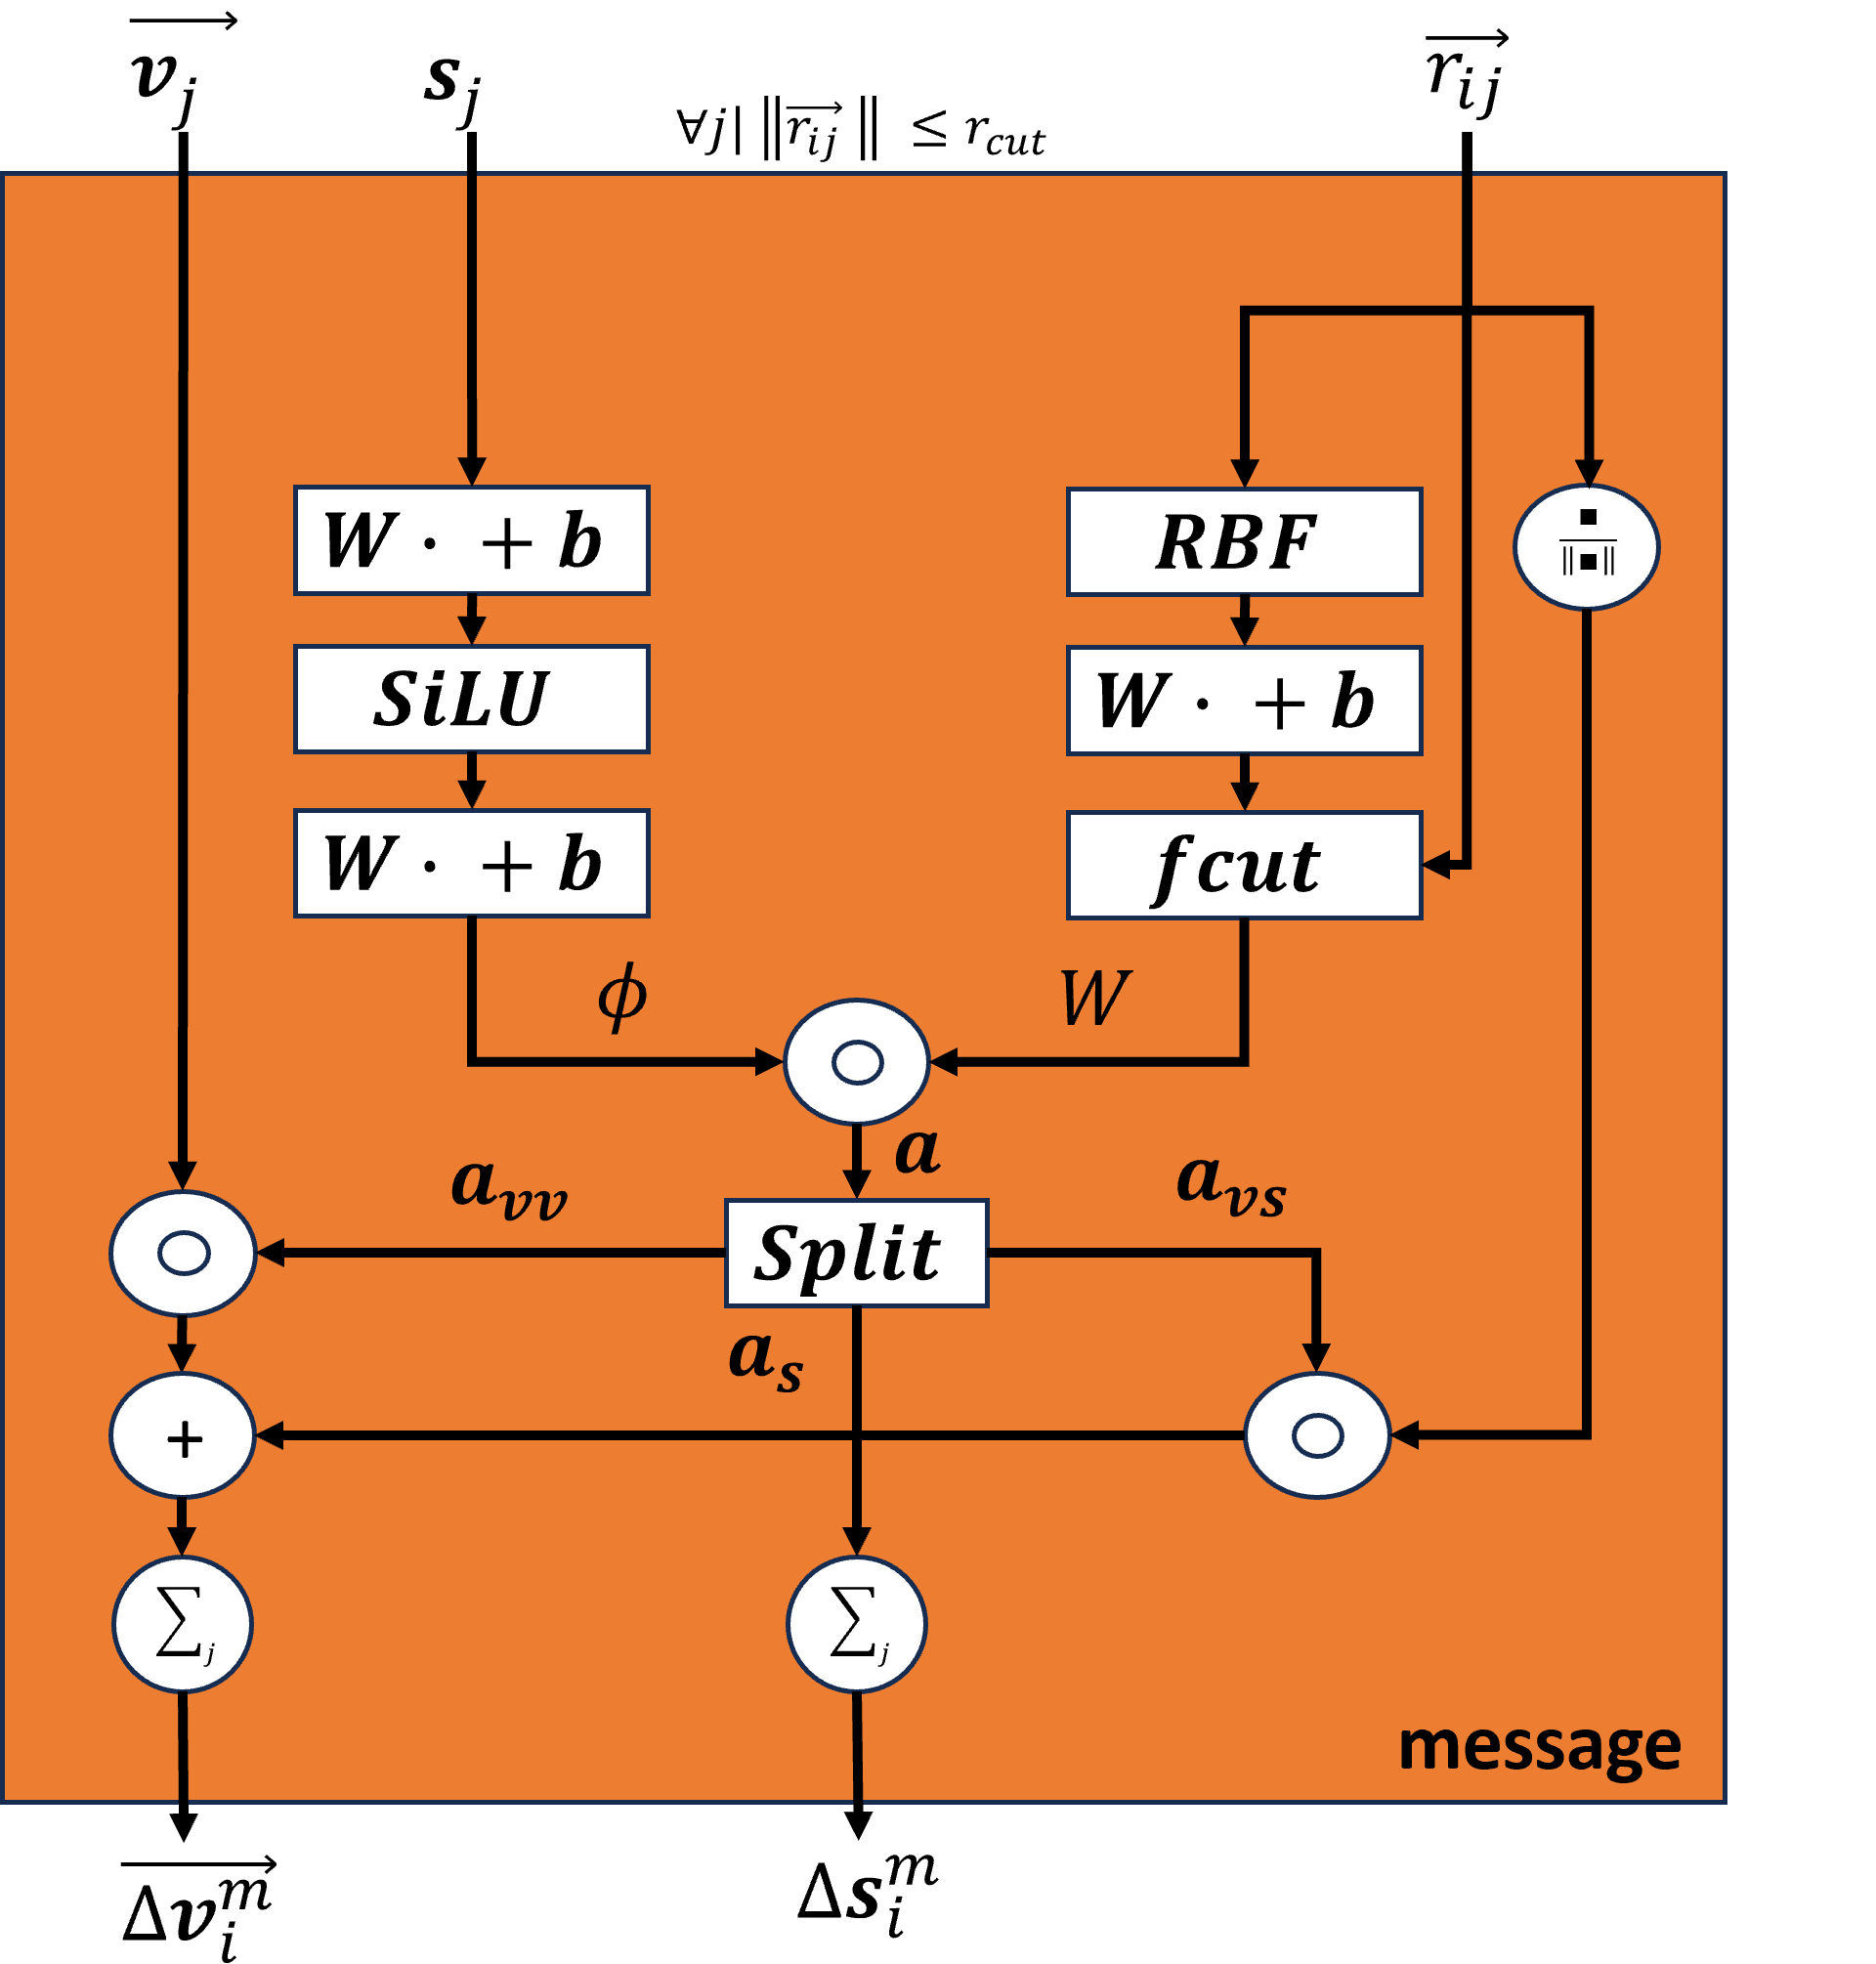
\includegraphics[width=250pt]{Images/Method/message_block.png}
\end{figure}

\subsubsection{Update Block}\label{subsubsec:update_block}

The update block builds on the information gained from the message block. It takes each individual node $n_{i} = (\mathbf{s}_{i}, \vec{\mathbf{v}}_{i})$
And runs ite through a set of transformations, before arriving at yet another set of residual update of the scalar and vector
representations respectively.

From the definition of an update function made in equation\ref{eq:residual_update}, the residual update of the invariant scalar properties
are defined for the update block as\ref{eq:residual_scalar_update}:

\begin{equation}\label{eq:residual_scalar_update}
    \Delta \mathbf{s}_{i}^{u}= \mathbf{a}_{ss} \left ( \mathbf{s}_{i}, \left \| \mathbf{V}\vec{\mathbf{v}}_{i} \right \| \right ) + \mathbf{a}_{sv} \left ( \mathbf{s}_{i}, \left \| \mathbf{V}\vec{\mathbf{v}}_{i} \right \| \right ) \left \langle \mathbf{U} \vec{\mathbf{v}}_{i}, \mathbf{V} \vec{\mathbf{v}}_{i} \right \rangle
\end{equation}

In general the update function, utilizes a shared network $a$, just as the message function did with $\phi$ and $\mathcal{W}$.
This network is defined as by inputs of the invariant scalar representation $\mathbf{s}_{i}$ and the normalized linear combination of
the equivariant vector representation $\left \| \mathbf{V}\vec{\mathbf{v}}_{i} \right \|$. both $U$ and $V$ are learned structures
by the network, and are applied inorder to produce the linear combinations of equivariant vector representations with dimensions:
$V \in \mathbb{R}^{F \times F}$ and $U \in \mathbb{R}^{F \times F}$.
The network applies two linear transformations
to the input $f$, as well a SiLU transformation $SiLU$. The full expression of $a$ can be seen in the following equation:
\begin{equation}\label{eq:a}
    \mathbf{a}(\mathbf{s}_{i}, \left \| \mathbf{V}\vec{\mathbf{v}}_{i} \right \|) = f_{4}(SiLU(f_{5}(\mathbf{s}_{i}, \left \| \mathbf{V}\vec{\mathbf{v}}_{i} \right \|)))
\end{equation}

The residual update of the scalar representations in the update block\ref{eq:residual_scalar_update} contains two terms.
The first term in\ref{eq:residual_scalar_update} relates to a non-linear scalar representation $\mathbf{a}_{ss} \left ( \mathbf{s}_{i}, \left \| \mathbf{V}\vec{\mathbf{v}}_{i} \right \| \right )$.
The second applies the scalar product of the two matrices $U$ and $V$, as further scaling to the non-linear of the invariant features $\mathbf{s_{i}}$,
as well as the coupling of the scalar representations with the normalized linear combination of the equivariant vector representation similar to the first
term. This whole expression imposes some further non-linearity on the scalar representations, as well as letting the equivariant representation
influence the output, via the scalar product, and the normalized linear combination.

The residual update of the vector representations in the update block is defined as\ref{eq:residual_vector_update}:

\begin{equation}\label{eq:residual_vector_update}
    \Delta \mathbf{v}_{i}^{u}= \mathbf{a}_{vv} \left ( \mathbf{s}_{i}, \left \| \mathbf{V}\vec{\mathbf{v}}_{i} \right \| \right ) \mathbf{U}\vec{\mathbf{v}}_{i}
\end{equation}

Which is similarly non-linear scaling $\mathbf{a}_{vv} \left ( \mathbf{s}_{i}, \left \| \mathbf{V}\vec{\mathbf{v}}_{i} \right \| \right )$
of the linear combinations of the equivariant representations, although the combinations are not normalized.

This concludes the section on the update block, a figure of the update-blocks architecture, can be found below\ref{img:update_block}.

\begin{figure}[H]
    \caption{Update block}
    \centering\label{img:update_block}
    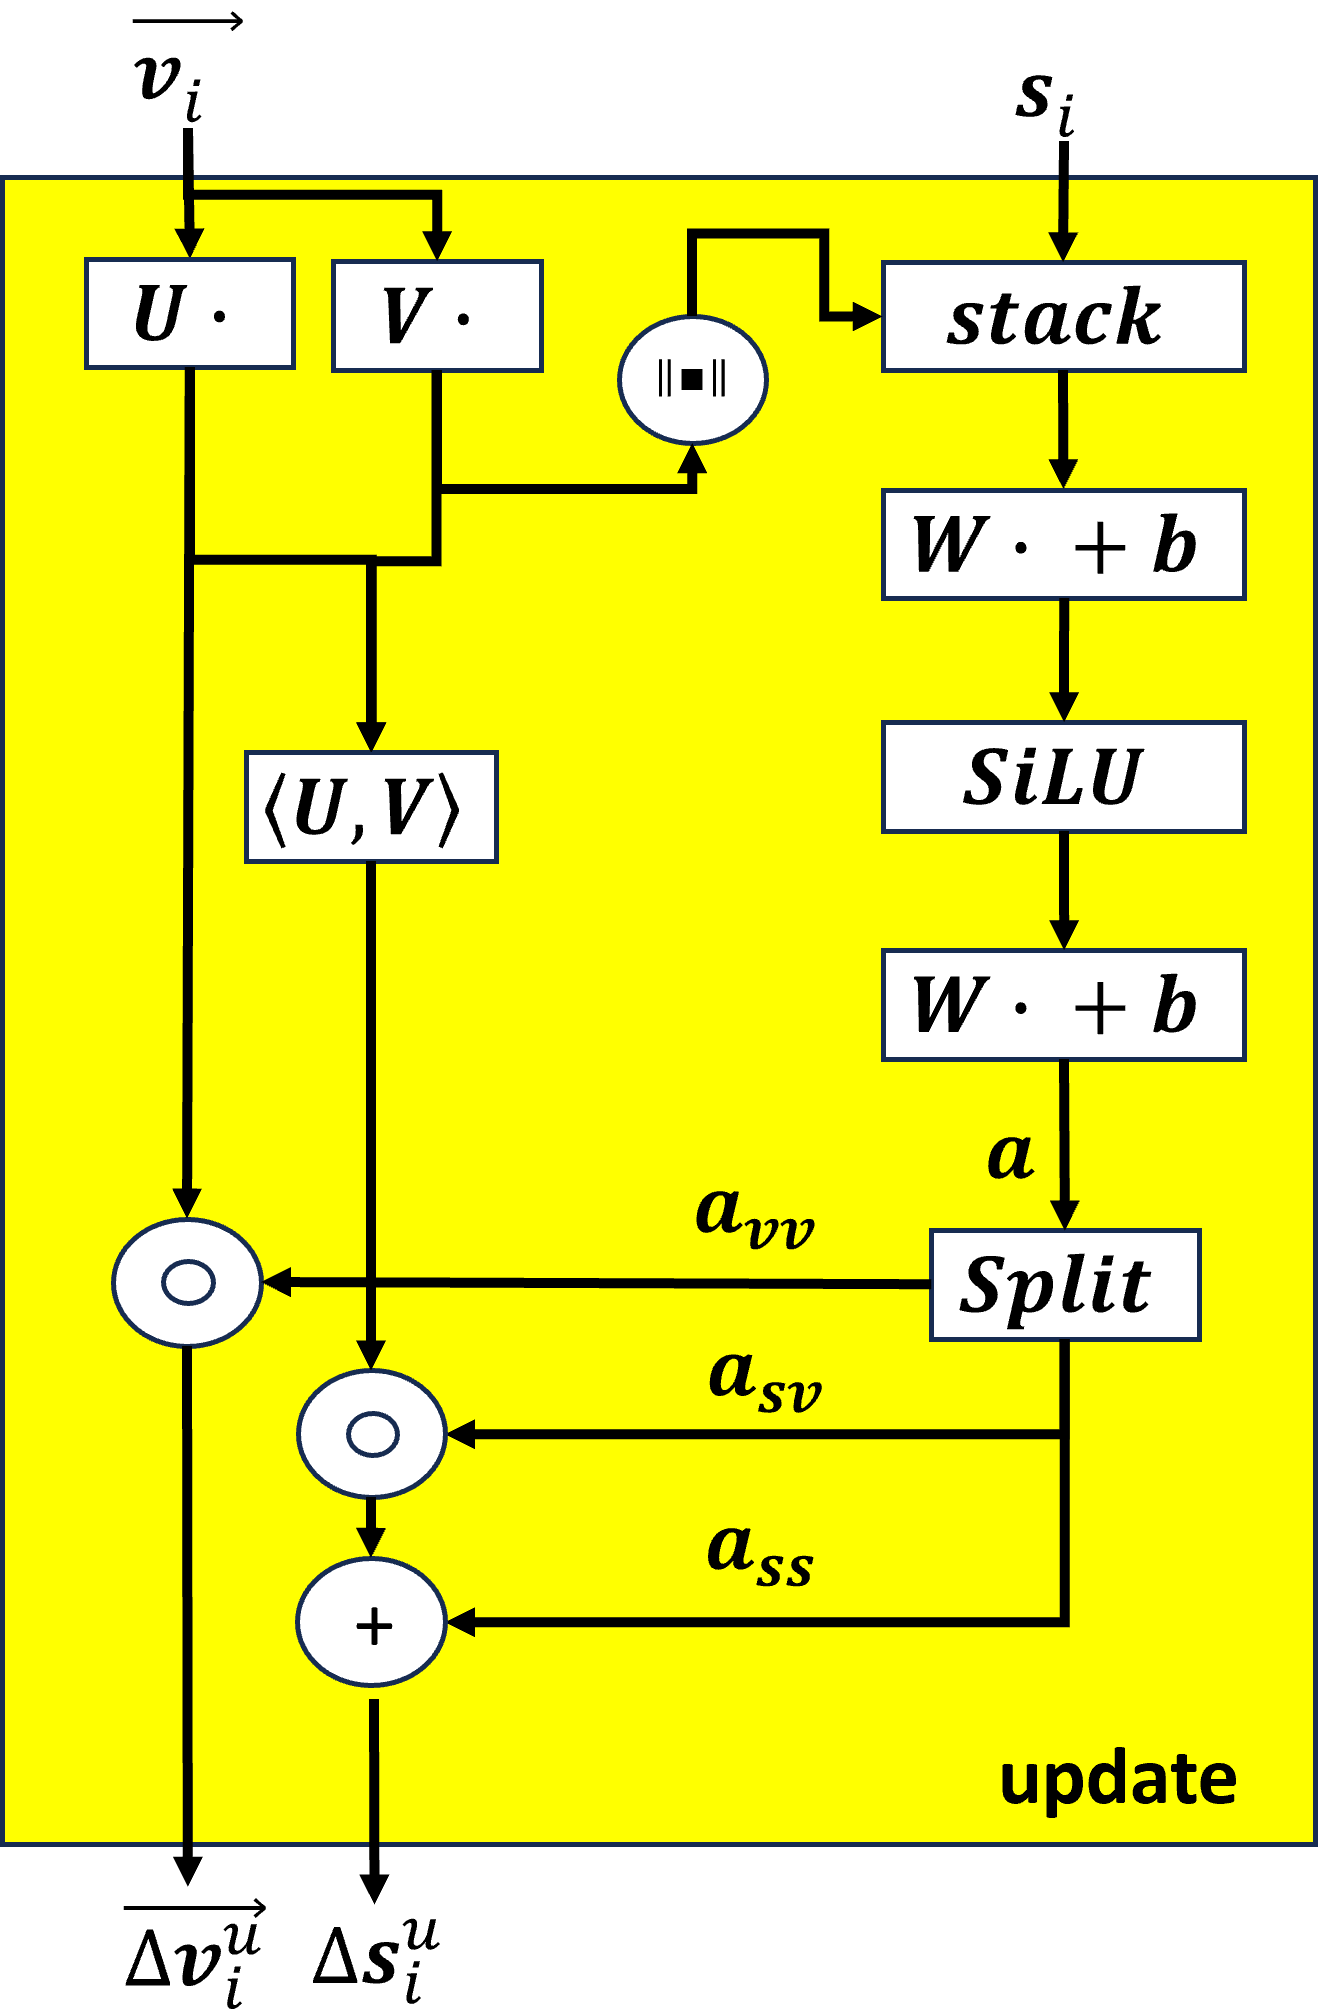
\includegraphics[width=200pt]{Images/Method/update_block.png}
\end{figure}

\subsubsection{A note on Equivariance}\label{note-equivariance}

As the initial symmetry section detailed\ref{sec:symmetry}, there are a number of operations which are valid for equivariant representations
of directional information. This section will take a short look back on the structures detailed above in the
message-\ref{subsubsec:message_block} and update-block\ref{subsubsec:update_block} sections, how exactly directional information
propagates in the network.

Directional information is propagated from vector differences $\vec{\mathbf{r}}_{ij}$ as input, into many of the model areas. The main storage
unit of directional information, is the equivariant vector representation $\vec{\mathbf{v}}_{i}$. This representation allows for directional
information to be stored across iterations, and it is therefore important that its equivariance characteristics are preserved.

If we take a look at the full set of operations applied to the vector representation, we can check for whether equivariance is preserved,
by checking the list presented in the section\ref{sec:symmetry}. The operations applied to the vector representation are as follows:

\begin{equation}\label{eq:vector_operations}
    \Delta \vec{\mathbf{v}}_{i} = \Delta \vec{\mathbf{v}}_{i}^{m} + \Delta \vec{\mathbf{v}}_{i}^{u} =
    \sum_{j} \vec{\mathbf{v}}_{j} \circ \phi_{vv}(\mathbf{s}_{j}) \circ \mathcal{W}_{vv} \left ( \left \| \vec{\mathbf{r}}_{ij} \right \| \right ) + \sum_{j} \phi_{vs}(\mathbf{s}_{j}) \circ \mathcal{W}'_{vs} \left ( \left \| \vec{\mathbf{r}}_{ij} \right \| \right ) \frac{\vec{\mathbf{r}}_{ij}}{\left \|\vec{\mathbf{r}}_{ij} \right \|} +
    \mathbf{a}_{vv} \left ( \mathbf{s}_{i}, \left \| \mathbf{V}\vec{\mathbf{v}}_{i} \right \| \right ) \mathbf{U}\vec{\mathbf{v}}_{i}
\end{equation}

we further break the expression down, into its seperate terms, we can analyse them one at a time:

\begin{equation}\label{eq:term-one}
    \sum_{j} \vec{\mathbf{v}}_{j} \circ \phi_{vv}(\mathbf{s}_{j}) \circ \mathcal{W}_{vv} \left ( \left \| \vec{\mathbf{r}}_{ij} \right \| \right )
\end{equation}

\begin{equation}\label{eq:term-two}
    \sum_{j} \phi_{vs}(\mathbf{s}_{j}) \circ \mathcal{W}'_{vs} \left ( \left \| \vec{\mathbf{r}}_{ij} \right \| \right ) \frac{\vec{\mathbf{r}}_{ij}}{\left \|\vec{\mathbf{r}}_{ij} \right \|}
\end{equation}

\begin{equation}\label{eq:term-three}
    \mathbf{a}_{vv} \left ( \mathbf{s}_{i}, \left \| \mathbf{V}\vec{\mathbf{v}}_{i} \right \| \right ) \mathbf{U}\vec{\mathbf{v}}_{i}
\end{equation}

The first term\ref{eq:term-one} scales the equivariant vector representation $\vec{\mathbf{v}}_{i}$, with a non-linear term, namely $\phi_{vv}(\mathbf{s}_{j})$, and
then further scales it with the rotationally invariant filter $\mathcal{W}_{vv}(\left \| \vec{\mathbf{r}}_{ij} \right \|)$. These two operations
are both listed in the section\ref{sec:symmetry}. Further, the summing over $j$, preserves the linearity, as long as the individual operations
are linear. Thus, equivariance is preserved. In the second term\ref{eq:term-two}, similar operations are applied to the unit vector produced from normalizing the
vector differences $\frac{\vec{\mathbf{r}}_{ij}}{\left \|\vec{\mathbf{r}}_{ij} \right \|}$. Two scalings of the vector, one non-linear, the other
by an invariant filter. Worth mentioning about the second term, is that it is a source of equivariant directional information.
The equivariant representation is
initialized, without directional information. The other terms either rely on directional information from the equivariant representation vector
or apply non-linear operations to directional information. The last term\ref{eq:term-three}, which is a non-linear scaling of linear-combinations
of the equivariant representation vector $\vec{\mathbf{v}}_{i}$. All operations listed in the above section, approved for preserving equivariance.

\subsubsection{Full Architecture}

The message- and update-blocks are coupled, and stacked, for input to pass through the blocks in a sequential manner. This sequence can be
seen in the figure below: \ref{img:MPNN_arc}


\begin{figure}[H]
    \caption{MPNN Full Architecture}
    \centering\label{img:MPNN_arc}
    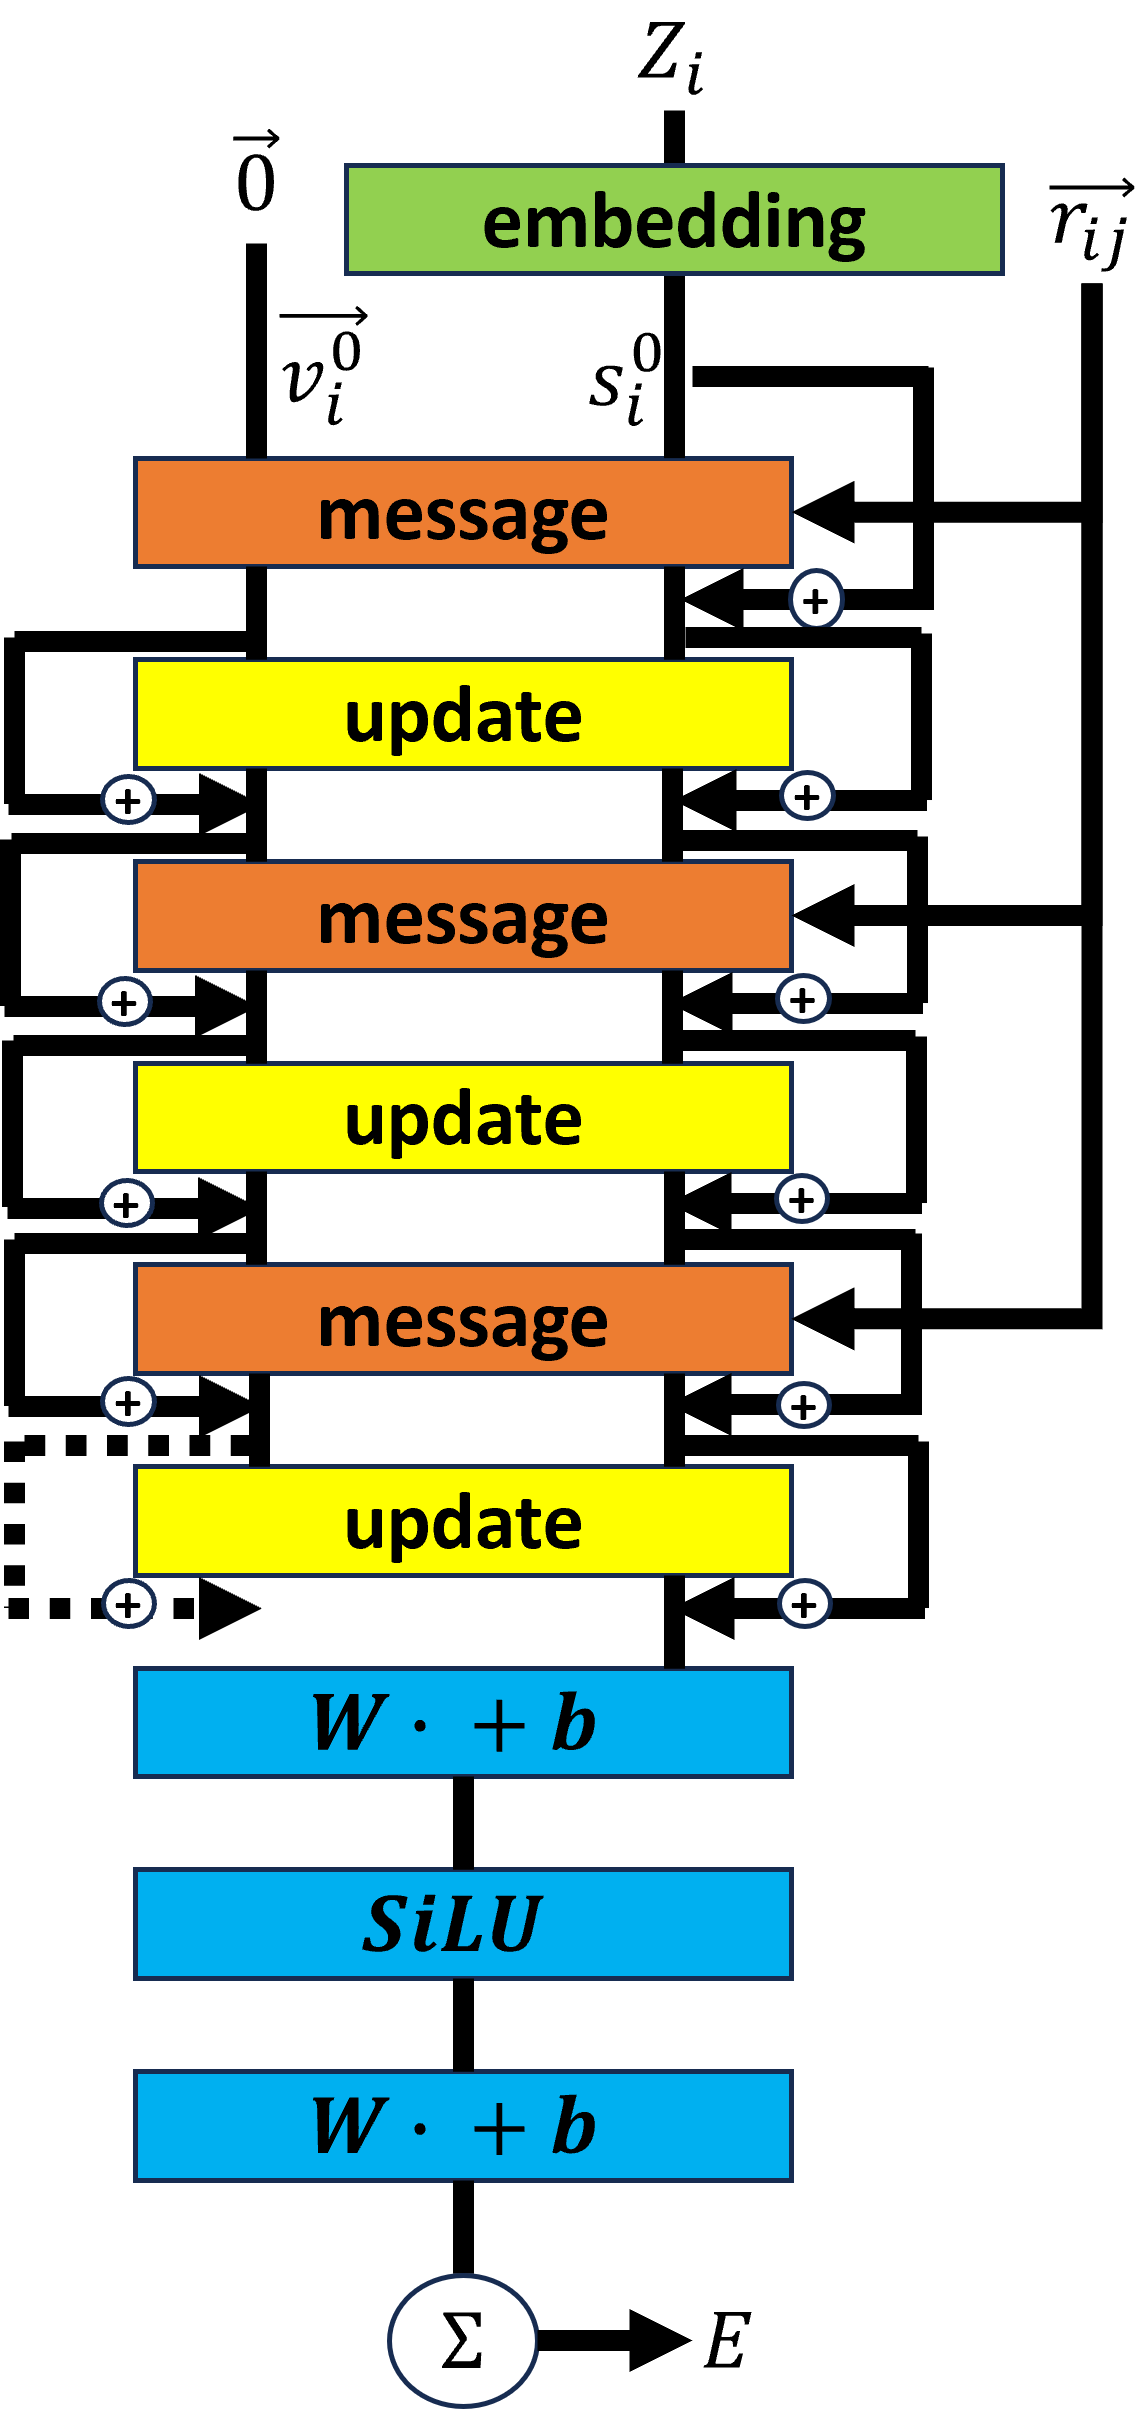
\includegraphics[width=150pt]{Images/Method/MPNN_arc.png}
\end{figure}

Worth noting about the full architecture, is the number of coupled message- and update-blocks, which is three. The output of these three
coupled sections will take the invariant scalar representations as input for a final set of layers, similar to the $\phi$-structure
presented earlier. Denote the scalar representations $\mathbf{s}_{i} \in \mathbb{R}^{F \times 1}$, the feature dimension $F$, utilizing the linear-layer-\ref{eq:linear_layer} and
SiLU\ref{eq:SiLU}-expressions from earlier. The expression of the output layer $O$ is then:

\begin{equation}
    \hat{\mathbf{y}} = \sum_{F} O(f_{6}(SiLU(f_{7}(\mathbf{s})))
\end{equation}

Which produces a set of predicted energies, which will be the output of the model. These output energies $\hat{\mathbf{y}}$, will be
compared to the targets of the model $\mathbf{y}$ to calculate the loss, via the mean squared error:

\begin{equation}\label{eq:loss}
    L = \frac{1}{N} \sum_{i=1}^N \left ( \hat{\mathbf{y}}_i - \mathbf{y}_i \right )^2
\end{equation}

This concludes the theoretical walkthrough of the inner workings of the implemented MPNN. The next section will detail the combination
of individual model architectures, into a bigger whole, namely an ensemble.

\subsection{Ensembles}

Ensembles (or Ensembling) is a technique for combining the predictive performance of individual modelling approaches
and to as an extension measuring uncertainty in the model. For the purpose of this study, only epistemic uncertainty, can be measured
in the models.

%#TODO MÅSKE: lav en figur der viser modeller som kombineres osv
In the context of MPNNs, ensembles can be created by training multiple models, in our case, on the same data set, 
with different initializations,
and combining their predictions to produce a mean and a variance among other metrics.
%#TODO Skriv noget mere her, omkring achored ensembles

\subsubsection{Descriptive statistics of the Ensemble}

Let $\mathbf{y}_i$ be the target binding energy for molecule $i$. Denote an ensemble of $T$ models where $t$ denotes a single model in the ensemble,
where $t \in \{1,2,\ldots,T\}$.
The ensemble prediction $\tilde{\mathbf{y}}_i$ can be calculated as the mean of the individual
model predictions $\mathbf{y}_{i,t}$, as done in\cite{Tran2019}, and proposed in \cite{Scalia2019}:

\begin{equation}\label{eq:mean-ensemble}
    \tilde{\mathbf{y}}_{i} = \frac{1}{T} \sum_{t=1}^{T} \mathbf{y}_{i,t}
\end{equation}

Further, in order to estimate the epistemic uncertainty in the ensemble predictions, we can calculate the variance based on individual model
predictions\cite{Tran2019}:

\begin{equation}\label{eq:variance-ensemble}
    \text{Var}(\mathbf{y}_{i}) = \frac{1}{T} \sum_{t=1}^T (\mathbf{y}_{i,t} - \tilde{\mathbf{y}}_i)^2
\end{equation}

\subsubsection{Uncertainty estimation}

Finally as the foundation of estimating uncertainty in the ensemble predictions, we can estimate the expected normal calibration error (ENCE).
This method relies on sorting metrics, in $K$ equal sized bins, where $k \in \{1,2,\ldots,K\}$ denotes a single bin.
A formal defintion of a bin is given below:
\begin{equation}\label{eq:bin}
    bin(x) = \begin{cases}
        1, & \text{if } x \text{ falls within the bin range} \\
        0, & \text{otherwise}
    \end{cases}
\end{equation}

Effectively outputting a result within a binary range, whether a given value, is within the bin range $1$, or outside the bin range $0$.

Further, we need to define a bin range. The bin ranges chosen are based on quantiles, which effectively will produce $K$ bins, of equal size.

Given a set of ascendingly sorted numbers $X = \{x_1, x_2, ..., x_n\}$ with $n$ elements. Denote a set of quantiles $P = \{p_0, p_1, ..., p_K\}$ with $K$ elements.
These quantiles are fractions of the number of elements in $X$ namely $n$ and the index $k$ of the element in $P$, specifically $\frac{p_{k}}{n}$.
The $p_{k}$-quantile of $X$, denoted as $Q(p_{k})$, is defined as follows:

\begin{itemize}
    \item Calculate the index of the quantile $q = p_{k} \cdot (n-1)$.
    \item If $q$ is an integer, $Q(p_{k})$ is equal to the $q$-th element of $X$, namely $x_{q}$.
    \item If $q$ is not an integer, $Q(p_{k})$ is equal to $\frac{1}{2} \cdot (x_{\lfloor q \rfloor} + x_{\lceil q \rceil})$
\end{itemize}

In the above, $\lceil \cdot \rceil$ and $\lfloor \cdot \rfloor$ denotes the ceiling and flooring functions respectively.
The ceiling function, denoted as $\lceil x \rceil$, rounds a real number $x$ up to the nearest integer greater than or equal to $x$. The flooring
function on the opposite, denoted as $\lfloor x \rfloor$, rounds a real number $x$ down to the nearest integer less than or equal to $x$.

These quantiles are then used to calculate the bin ranges:
\begin{equation}\label{eq:binrange}
    binrange(k) = \left[ Q(p_{k}); Q(p_{k+1}) \right]
\end{equation}

So for the final definition of the bin, utlizing the quantiles to produce bin ranges.

\begin{equation}\label{eq:bin-k}
    bin_{k}(x) = \begin{cases}
        1, & \text{if } x \in binrange(k) \\
        0, & \text{otherwise}
    \end{cases}
\end{equation}

Utilizing the above definition of a bin, we now want to sort all errors made by the individual models $e = y_{i} - {y}_{i,t}$ in ascending fashion.
We now define $K = \{1,2,\ldots,K\}$ bins, and $P = \{p_0, p_1, ..., p_K\}$ quantiles for the error metric to be sorted into bins.
the sorting is done via the below expression for all $k \in \{1,2,\ldots,K\}$ and all models $t \in \{1,2,\ldots,T\}$:

\begin{equation}\label{eq:bin-error}
    bin_{k}(e) =\begin{cases}
        1, & \text{if } e \in binrange(k) \\
        0, & \text{otherwise}
    \end{cases}
\end{equation}

We now wish to calculate the root mean squared error (RMSE) on each bin. The RMSE metric, describes the mean of empirical error, made
by all the models in the given bin. 
Denote the number of elements in the bin as $N$, where the
expression of the RMSE, is as follows:

\begin{equation}
    RMSE_{k} = \sqrt{\frac{1}{N} \sum_{n=1}^N \left( e_{n,k} \right)^2}
\end{equation}

We now go through a similar process, for differences between individual predictions and the means of the predictions 
$d = y_{i,t} - \tilde{y}_{i}$. We sort them in ascending order. Define $K = \{1,2,\ldots,K\}$ bins, and $P = \{p_0, p_1, ..., p_K\}$ 
quantiles for the difference metric to be sorted into. the sorting is done via the below expression for all $k \in \{1,2,\ldots,K\}$ 
and all models $t \in \{1,2,\ldots,T\}$:

\begin{equation}\label{eq:bin-difference}
    bin_{k}(d) =\begin{cases}
        1, & \text{if } d \in binrange(k) \\
        0, & \text{otherwise}
    \end{cases}
\end{equation}

Now wanting to produce the root mean variance (RMV) on each bin. The RMV metric, describes the variance on predictions, made
by all the models in the given bin.
Denote the number of elements in the bin as $N$, where the
expression of the RMV, is as follows:

\begin{equation}
    RMV_{k} = \sqrt{\frac{1}{N} \sum_{n=1}^N  d_{n,k}}
\end{equation}

We now wish to produce the ENCE-metric\ref{eq:calibration-error}\cite{Busk2021}.
This metric is produced based on the RMSE and RMV metrics, calculated further above.
These metrics are calculated for each $k$-bin, for the chosen number of bins $K$. The ENCE metric
is defined below, followed by the RMSE and the RMV.

\begin{equation}\label{eq:calibration-error}
    ENCE = \frac{1}{k} \sum_{k=1}^K \frac{|RMV_{k} - RMSE_{k}|}{RMV_{k}}
\end{equation}

These methods are heavily inspired by the methods in the papers\cite{Tran2019} and \cite{Busk2021}. Elements and approaches have been 
drawn from both, effectively doing cherrypicking for the scope of this project. The approach by Busk2021, is on models with two output
metrics, compared to this projects one. The paper by Tran2019, utilizes a similar approach to describing epistemic uncertainty in the
ensemble predictions, made by models with one output metric. But tran2019, lacks in the descriptive metrics that Busk2021 has, i.e 
RMSE, RMV, and ENCE.


\newpage